\documentclass[../main.tex]{subfiles}
\graphicspath{
    {"../img/"}
    {"img/"}
}

\begin{document}
\subsection{Formy różniczkowe}
(czyli o uprawianiu analizy na powierzchni balonika albo kartki)

Niech $M\subset\mathbb{R}^n$ - taki, że dla każdego punktu $p\in M$ istnieje otoczenie otwarte $U\subset M$
\begin{przyklad}
    (sfera, obwarzanek, itd., okrąg), (stożek - nie ok!), (taka ósemka co się przecina - też nie)
\end{przyklad}
\begin{definicja}
Niech $U$ - zbiór otwarty $\subset M$ i niech odwzorowanie $\varphi: U\to \mathbb{R}^n$ takie, że $\varphi$ - klasy $\mathcal{C}^1$, (czasami $\mathcal{C}^\infty$ ), $\varphi^{-1}$ - klasy $\mathcal{C}^1$, (czasami $\mathcal{C}^\infty$ ) nazywamy mapą.\\
Uwaga: mapa \underline{nie musi} pokrywać całego zbioru $M$.
\end{definicja}

Wyobraźmy sobie, że mamy jakiś zbiór $M$. Połowa tego zbioru to niech będzie $U_1$, i ono się przecina z $U_2$. $U_1$ i $U_2$ możemy rozłożyć na prostokąty w $\mathbb{R}^2$. Co się stanie z punktami mapowanymi do obu $U$?
\begin{definicja}
    $(U^1,\varphi^1), (U^2,\varphi^2)$ - mapy na $M$.\\
    $U_1$ i $U_2$ nazywamy zgodnymi jeżeli\\
    $a)$ $U_1\cap U_2 = \phi$\\
    albo odwzorowanie $\varphi_2 \circ \varphi_1^{-1}: \varphi_1(U_1\cap U_2)\to \varphi_2(U_2\cap U_1)$ jest bijekcją (klasy powiedzmy sobie $\mathcal{C}^1, \mathcal{C}^{\infty}$ )
\end{definicja}
    \begin{figure}[h]
        \centering
        \includegraphics[width=0.5\textwidth]{fig_49}
        \caption{$M = \left\{ (x,y): x^2 + y^2 = 1^2 \right\}$}
    \end{figure}
\begin{przyklad}
    \begin{align*}
    &U_1 = \left\{ (x,y)\in M, y>0 \right\},\quad \varphi_1: (x,y)\in U_1 \to x\\
    &U_2 = \left\{ (x,y)\in M, x>0 \right\},\quad \varphi_2: (x,y)\in U_2 \to y\\
    &U_3 = \left\{ (x,y)\in M, y<0 \right\},\quad \varphi_3: (x,y)\in U_3 \to x\\
    &U_4 = \left\{ (x,y)\in M, x<0 \right\},\quad \varphi_4: (x,y)\in U_4 \to y
    .\end{align*}
    $U_1$ i $U_3$ oraz $U_2$ i $U_4$ są zgodne. Czy zgodne są $U_1$ i $U_2$? Czyli chcemy zbadać odwzorowanie $\varphi_1(U_1\cap U_2)\to \varphi_2(U_1\cap U_2)$, ale $\varphi_1(x,y)\in U_1\to x$.\\
    Czyli $\varphi_1^{-1}(x)\to \left( x, \sqrt{1-x^2}  \right) $,\\
    czyli $\varphi_2(\varphi_1^{-1}(x) = \varphi_2((x,\sqrt{1-x^2} )) = \sqrt{1-x^2} $.\\
    Zatem czy $\varphi_2 \circ \varphi_{1}^{-1}(x) = \sqrt{1-x^2} $ przerzuca $]0,1[\to]0,1[$ jest różniczkowalne? Odpowiedź: na zbiorze $]0,1[$ jest.
\end{przyklad}
\begin{definicja}
    Kolekcję zgodnych map nazywamy atlasem. Zbiór $M$ wraz z atlasem, który pokrywa cały $M$ nazywamy \textbf{rozmaitością} (\textit{ang. manifold}).
\end{definicja}

\end{document}

